\documentclass[10pt,a4paper]{article}
\usepackage[utf8]{inputenc}
\usepackage{amsmath}
\usepackage{amsfonts}
\usepackage{amssymb}
\usepackage{graphicx}
\usepackage[margin=1in]{geometry}  
\usepackage{float}
\usepackage{caption}
\usepackage{subcaption}
\begin{document}

\section*{Task 1 - Unknown Intrinsic and Extrinsic Parameters}

Without knowing any of the parameters for the image capture device, it is very hard to keep the images aligned or to keep projective form. The images are quite distorted, but corresponding points do match up along horizontal lines. Without any camera parameters, we are only able to reconstruct a scene up to a projective transformation.

\begin{figure}[h]
\centering
\begin{subfigure}{.5\textwidth}
  \centering
  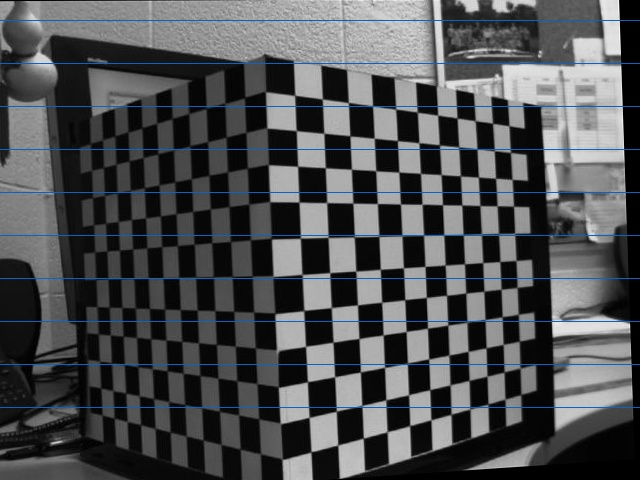
\includegraphics[height=4cm,keepaspectratio]{paraCubeS}
  \caption{Start}
  \label{fig:sub1}
\end{subfigure}%
\begin{subfigure}{.5\textwidth}
  \centering
  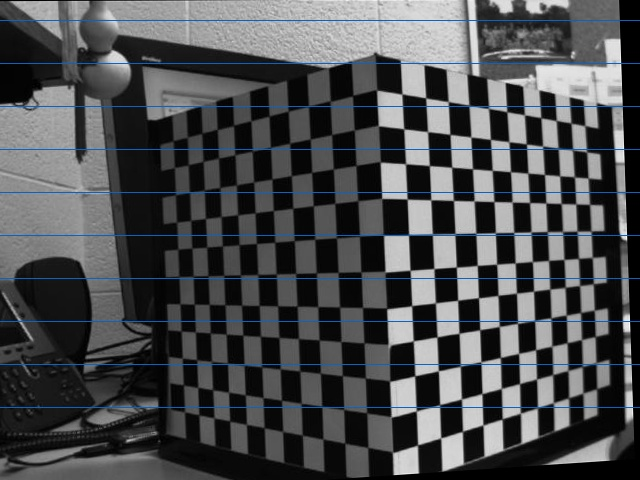
\includegraphics[height=4cm,keepaspectratio]{paraCubeE}
  \caption{End}
  \label{fig:sub2}
\end{subfigure}
\label{fig:test}
\caption{Parallel Cube}
\end{figure}

\begin{figure}[h]
\centering
\begin{subfigure}{.5\textwidth}
  \centering
  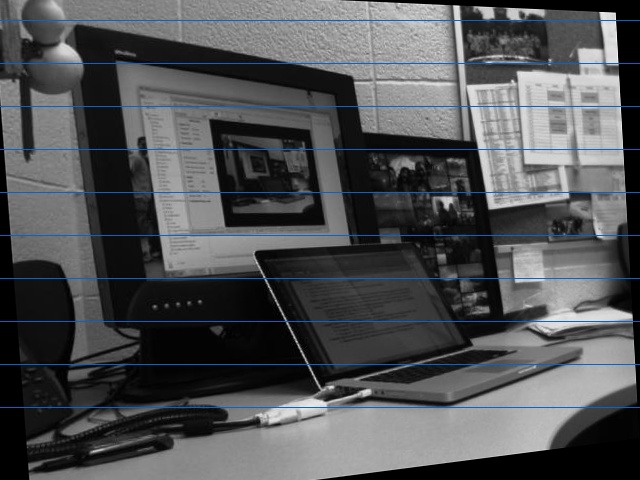
\includegraphics[height=4cm,keepaspectratio]{paraRealS}
  \caption{Start}
  \label{fig:sub1}
\end{subfigure}%
\begin{subfigure}{.5\textwidth}
  \centering
  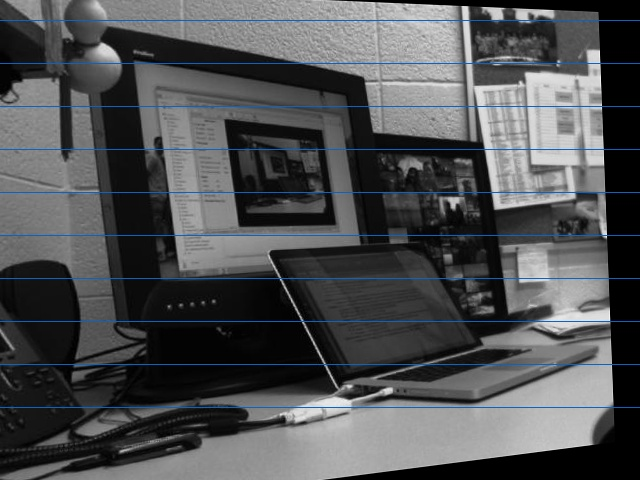
\includegraphics[height=4cm,keepaspectratio]{paraRealE}
  \caption{End}
  \label{fig:sub2}
\end{subfigure}
\label{fig:test}
\caption{Parallel Real}
\end{figure}

\begin{figure}[h]
\centering
\begin{subfigure}{.5\textwidth}
  \centering
  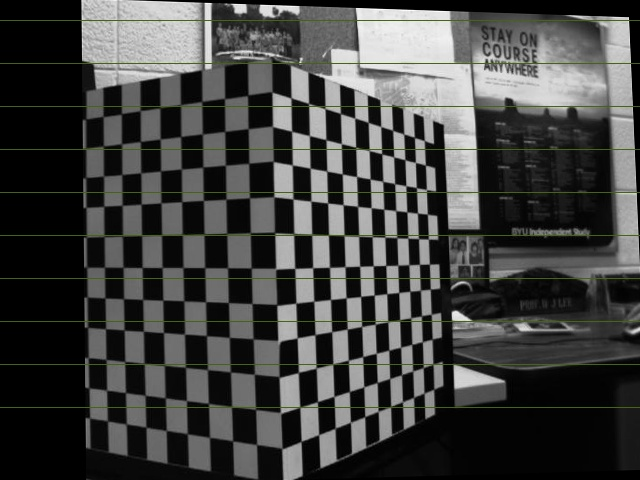
\includegraphics[height=4cm,keepaspectratio]{turnCubeS}
  \caption{Start}
  \label{fig:sub1}
\end{subfigure}%
\begin{subfigure}{.5\textwidth}
  \centering
  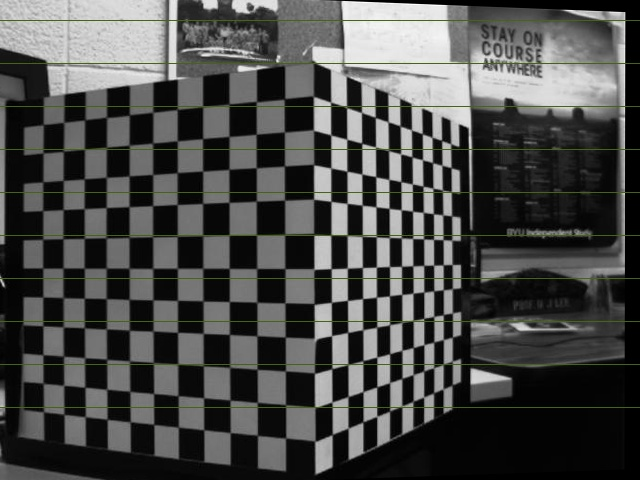
\includegraphics[height=4cm,keepaspectratio]{turnCubeE}
  \caption{End}
  \label{fig:sub2}
\end{subfigure}
\label{fig:test}
\caption{Turned Cube}
\end{figure}

\begin{figure}[h]
\centering
\begin{subfigure}{.5\textwidth}
  \centering
  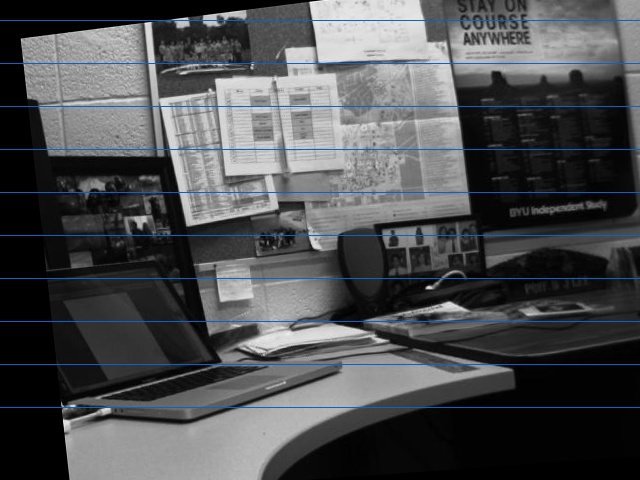
\includegraphics[height=4cm,keepaspectratio]{turnRealS}
  \caption{Start}
  \label{fig:sub1}
\end{subfigure}%
\begin{subfigure}{.5\textwidth}
  \centering
  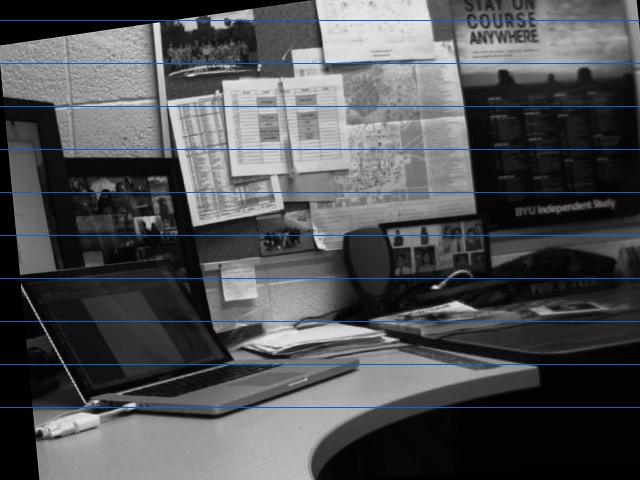
\includegraphics[height=4cm,keepaspectratio]{turnRealE}
  \caption{End}
  \label{fig:sub2}
\end{subfigure}
\label{fig:test}
\caption{Turned Real}
\end{figure}

\section*{Task 2 - Known Intrinsic Parameters}
It is observed that the decomposition of the fundamental matrix creates motion that makes good sense. We can play the sequence of images and see readily that the camera is moving from right to left, essentially entirely in the x-direction. When the fundamental matrix is decomposed correctly, we see this same behavior, up to a scale factor. The math is such that the transformation vector has a norm of 1. 

The rotation matrices largely appear to be very very close to the identity matrices. The only exception that deviates significantly is in the turned real sequence, which would be understandable that the camera turns somewhat. 

The following are the R, T, E, and F matrices for each type of transformation: 

\textbf{Parallel Real}

F -- parallel real: 
\begin{equation*}
\begin{bmatrix}
-4.29676e-07 & 0.000150455 & -0.0132263 \\ -0.000137004 & -7.04904e-06 & -0.424941 \\ 0.0109562 & 0.417858 & 1
\end{bmatrix}
\end{equation*}

E -- parallel real: 
\begin{equation*}
\begin{bmatrix}
-0.0011441 & 0.256827 & 0.0494144 \\ -0.232793 & -0.00627945 & -0.971162 \\ -0.0506966 & 0.965185 & -0.00758867
\end{bmatrix}
\end{equation*}

R -- parallel real: 
\begin{equation*}
\begin{bmatrix}
-0.9997 & 0.000256749 & -0.0244807 \\ -0.000417606 & -0.999978 & 0.00656588 \\ 0.0244785 & -0.00657414 & -0.999679
\end{bmatrix}
\end{equation*}

T -- parallel real: 
\begin{equation*}
\begin{bmatrix}
0.965193 & 0.051115 & -0.256497
\end{bmatrix}
\end{equation*}

\textbf{Parallel Cube}

F -- parallel cube: 
\begin{equation*}
\begin{bmatrix}
2.16243e-07 & 1.50848e-05 & -0.00938923 \\ -4.44753e-06 & 4.22347e-06 & -0.318471 \\ 0.00728704 & 0.313221 & 1
\end{bmatrix}
\end{equation*}

E -- parallel cube: 
\begin{equation*}
\begin{bmatrix}
0.000559038 & 0.0388508 & -0.0170599 \\ -0.0116103 & 0.00553807 & -0.999768 \\ 0.0195876 & 0.999039 & 0.00597645
\end{bmatrix}
\end{equation*}

R -- parallel cube: 
\begin{equation*}
\begin{bmatrix}
-0.999628 & 0.00246471 & -0.027144 \\ -0.0023159 & -0.999982 & -0.00551236 \\ 0.0271571 & 0.00544745 & -0.999616
\end{bmatrix}
\end{equation*}

T -- parallel cube: 
\begin{equation*}
\begin{bmatrix}
0.999099 & -0.0172802 & -0.0387574
\end{bmatrix}
\end{equation*}

\textbf{Turned Real}

F -- turned real: 
\begin{equation*}
\begin{bmatrix}
-5.64669e-07 & 4.34349e-05 & -0.0220842 \\ -3.6285e-05 & 2.06365e-06 & 0.138153 \\ 0.0202722 & -0.141181 & 1
\end{bmatrix}
\end{equation*}

E -- turned real: 
\begin{equation*}
\begin{bmatrix}
-0.00321248 & 0.272316 & -0.087248 \\ -0.228974 & 0.00998507 & 0.969691 \\ 0.0822613 & -0.958434 & 0.00543935
\end{bmatrix}
\end{equation*}

R -- turned real: 
\begin{equation*}
\begin{bmatrix}
-0.85993 & -0.164906 & -0.483038 \\ -0.161844 & 0.98563 & -0.0483654 \\ -0.484073 & -0.0365857 & 0.874263
\end{bmatrix}
\end{equation*}

T -- turned real: 
\begin{equation*}
\begin{bmatrix}
0.958239 & 0.0846855 & 0.273143
\end{bmatrix}
\end{equation*}

\textbf{Turned Cube}

F -- turned cube: 
\begin{equation*}
\begin{bmatrix}
1.69916e-08 & 8.73677e-06 & -0.00253715 \\ -4.82891e-06 & 5.61749e-06 & -0.0834156 \\ 0.00154827 & 0.0778403 & 1
\end{bmatrix}
\end{equation*}

E -- turned cube: 
\begin{equation*}
\begin{bmatrix}
0.000290298 & 0.0872629 & -0.00138408 \\ -0.0477024 & 0.0274256 & -0.998478 \\ 0.00538237 & 0.995799 & 0.0274246
\end{bmatrix}
\end{equation*}

R -- turned cube: 
\begin{equation*}
\begin{bmatrix}
0.990856 & -0.00543455 & -0.134813 \\ -0.00915855 & -0.999593 & -0.0270186 \\ -0.134611 & 0.0280063 & -0.990503
\end{bmatrix}
\end{equation*}

T -- turned cube: 
\begin{equation*}
\begin{bmatrix}
0.996184 & -0.00377576 & -0.0871926
\end{bmatrix}
\end{equation*}

\section*{Task 3 - Known Extrinsic and Intrinsic Parameters}

In order to find the scale factor, I made code where I could select a ROI around the leading edge of each cube by using a mouse event handler. I then found the Z values for all of these points (using their corresponding points I had loaded in from the last task), and found the closest z-value. I then found the scale factor by dividing 20 by this Z factor, which then means that all of the points in an image can be scaled by that factor. I scaled the translations in each image by this scale factor, with this result (all measurements are in inches): 

\textbf{Turned Cube T}

\begin{equation*}
\begin{bmatrix}
9.22723 & -0.03497 & -0.80762
\end{bmatrix}
\end{equation*}

\textbf{Parallel Cube T} 

\begin{equation*}
\begin{bmatrix}
13.1852& -0.2280& -0.51148
\end{bmatrix}
\end{equation*}

\textbf{Turned Real T} 

\begin{equation*}
\begin{bmatrix}
8.8757& 0.784405& 2.5300
\end{bmatrix}
\end{equation*}

\textbf{Parallel Real T} 

\begin{equation*}
\begin{bmatrix}
12.7377& 0.67457& -3.3850
\end{bmatrix}
\end{equation*}


I also chose random points in the image, found their 3D information, and drew them on the image. For convenience, I also wrote the number corresponding to each point on the image by the point. Some of the points may not correlate very well because, due to the random points, some may not have been tracked as precisely.  

\textbf{Parallel Cube}

\begin{figure}[H]
\centering
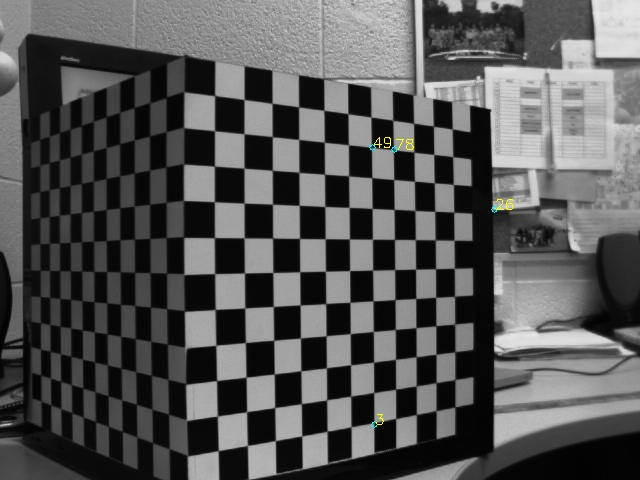
\includegraphics[height=7cm,keepaspectratio]{parallelCube_3dinfo}
\caption{Parallel Cube}
\end{figure}

Real-world xyz coordinates for point 3 are 11.2461, 12.7511, 24.7864

Real-world xyz coordinates for point 26 are 11.9565, 5.0493, 19.9743

Real-world xyz coordinates for point 49 are 11.2366, 4.43982, 24.9452

Real-world xyz coordinates for point 78 are 11.3703, 4.30705, 23.8204

\textbf{Turned Cube}

\begin{figure}[H]
\centering
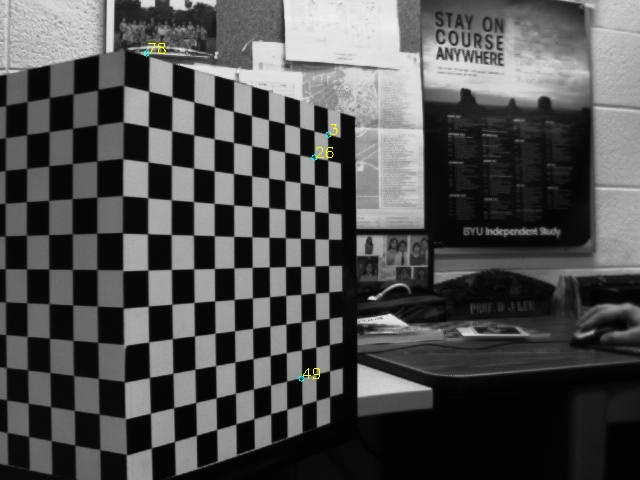
\includegraphics[height=7cm,keepaspectratio]{turnCube_3dinfo}
\caption{Turned Cube}
\end{figure}

Real-world xyz coordinates for point 3 are 7.67408, 3.13125, 19.3248

Real-world xyz coordinates for point 26 are 7.59514, 3.80491, 19.9467

Real-world xyz coordinates for point 49 are 7.59404, 9.52815, 20.7812

Real-world xyz coordinates for point 78 are 6.17592, 2.25641, 34.9383

\textbf{Parallel Real}

\begin{figure}[H]
\centering
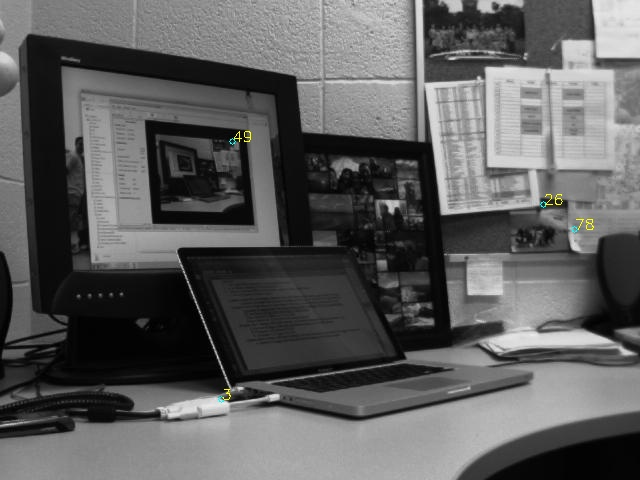
\includegraphics[height=7cm,keepaspectratio]{parallelreal_3dinfo}
\caption{Parallel Real}
\end{figure}

Real-world xyz coordinates for point 3 are 11.3698, 20.5212, 42.4328

Real-world xyz coordinates for point 26 are 14.2449, 5.36123, 21.6319

Real-world xyz coordinates for point 49 are 11.8756, 7.21613, 42.1685

Real-world xyz coordinates for point 78 are 14.3983, 5.73535, 20.696

\textbf{Turned Real}

\begin{figure}[H]
\centering
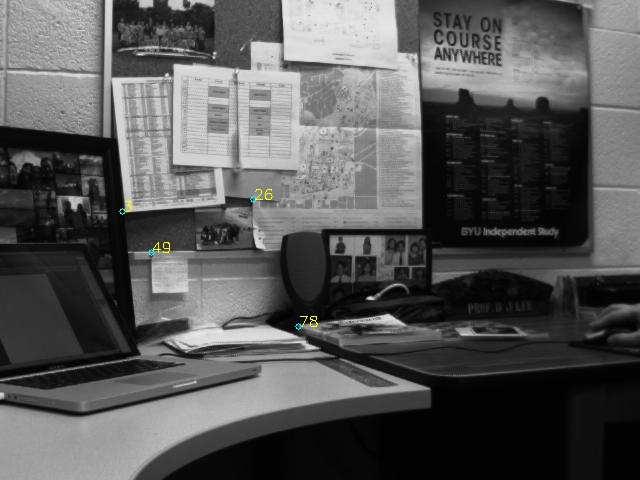
\includegraphics[height=7cm,keepaspectratio]{turnReal_3dinfo}
\caption{Turned Real}
\end{figure}

Real-world xyz coordinates for point 3 are 6.94562, 11.9894, 46.8938

Real-world xyz coordinates for point 26 are 9.25938, 7.29853, 30.2007

Real-world xyz coordinates for point 49 are 7.29249, 12.2138, 39.9596

Real-world xyz coordinates for point 78 are 9.00928, 9.8619, 24.9461



\end{document}